\documentclass{article}
\usepackage{booktabs}
\usepackage{indentfirst}
\usepackage{graphicx}
\usepackage[style=apa,backend=biber,doi=false,isbn=false,url=false,eprint=false]{biblatex}
\DeclareLanguageMapping{english}{american-apa}
\addbibresource{./.resources/biblatex.bib}

\usepackage{float}
\usepackage{todonotes}
\begin{document}

\section{A Historical View on Myanmar}

The political situation in Myanmar has always been chaotic. Since gaining independence from British colonial rule in 1948, coups, uprisings, and revolutions have been occurring constantly. By the time this paper is being written, Myanmar has just gone through a political unrest, labeled as \textit{Operation 1027}. The Three Brotherhood Alliance, composed of the Arakan Army, the Myanmar National Democratic Alliance Army, and the Ta’ang National Liberation Army, rebelled against the junta and eventually seized control over Shan State.\autocite{yunsunOperation1027Changing2024} This operation's impact extended beyond Shan State, inspiring offensives in other regions such as Kachin and Sagaing. In Kachin State, for instance, the Cochin Independence Army (KIA) attacked and overran strategic locations, leadin:g to significant confrontations with the Myanmar armed forces.\autocite{theinternationalinstituteforstrategicstudiesOperation1027Reshapes2023} However, the details of this operation are not our main interest here. What concerns us is the reason such uproar occurs.

The official account claims that the junta's oppression and the people's rage caused this coup.\autocite{htetminlwinOperation1027End2023} I believe this claim to be oversimplified and unsuccessful. No government intends to be evil, and even if there is a conflict of interest between the government and the people, the strife should not have lasted for such a long period. In the following section, I will propose an alternative reason for explaining such conflict. I argue that the problem stems from historical reasons by giving an account of a continuous struggle between different ethnic groups in Myanmar.

\subsection{Precolonial Period}

The nature of southeast Asian politics itself has its own character, which \textcite{tambiahGalacticPolity2007} called ``The Galactic Polity''. This idea comes from ``mandalas,'' originally reflecting how people thought the universe was organized (see figure \ref{mandala}). Accordingly, ancient Southeast Asian societies arranged their cities and kingdoms like mandalas, with the authority in the center and other important places around it. 

The consequence of such arrangement is that the control is hierarchical but decentralized. Local rulers maintained a degree of autonomy within the overarching framework of the central authority. Another feature of model is its flexibility. Instead of expanding and guarding borders, it is more like appending nodes to a tree. This reflexes the fluid and adaptable nature of political authority and territorial control in Southeast Asia. \textcite{liebermanEthnicPoliticsEighteenthCentury1978} points out that such fluidity makes conflicts even goes deeper than ethnic identity like Peg, Ava or Burma. The scope of this paper, however, would go no further than the classical account of ethnic conflict and leave Lieberman's theory for future analysis.

\begin{figure}[H]
        \centering
        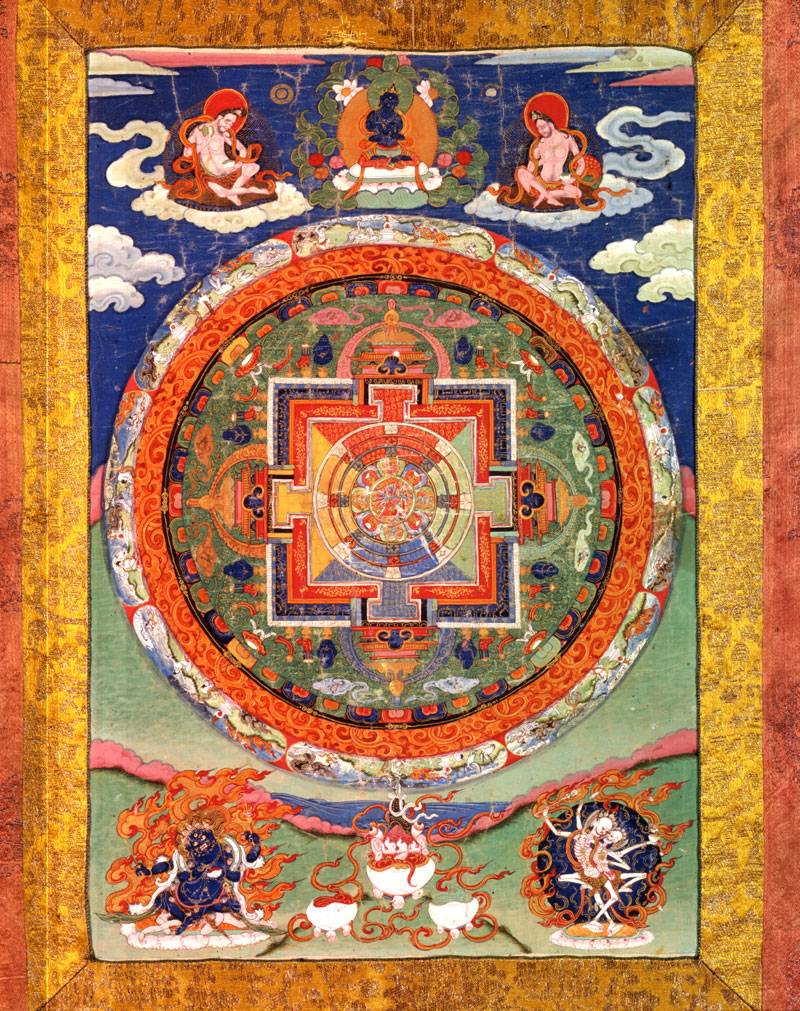
\includegraphics[width=\textwidth]{mandala.png}
        \caption{\cite{
This is especially true for Myanmar. Historically, Myanmar hosts approximately seven major and many more minor ethnic-linguistic groups, nearly all of whom belong to three of the four main language families of Southeast Asia: Tibet-Burman, Tai-Kadai, Austro-Asiatic, and Austronesian. The ethnic groups such as the Shan, Arakanese, and Mon have played significant roles in history. \autocite[p.46-56]{aung-thwinHistoryMyanmarAncient2012} Especially, over 40 different sub-states evolved within the Shan State. They are ruled by royal Sawbwa who rivalled the powers of the Burman kings.\autocite[18,54]{smithEthnicGroupsBurma1994} 

Geographically speaking, the most significant gap, both politically and culturally, is the gap between Upper Myanmar (dry zone, centered around the Irrawaddy River Valley) and Lower Myanmar (the delta region). The term in Burmese, anya (`upstream') and akye (`downstream') already reflects that it is not only a geographical distinction, but also a cultural one. Anyatha (`offspring of the upstream region’) would consider akyitha(`offspring of the downstream region’) as unintelligent and peculiar. \autocite[43,142]{aung-thwinHistoryMyanmarAncient2012}

The gap lies also economically. Lower Myanmar's historical development and culture were influenced significantly by international and regional trade in the Gulf of Muttama (Martaban) and the Bay of Bengal. This exposure to external influences made Lower Myanmar demographically and culturally diverse, adaptable, and less homogeneous ethno-linguistically. In contrast, Upper Myanmar's prosperous agriculture demands a stable society, and thus it is more inwards and homogeneous. Before the colonization, Upper and Lower Myanmar are only united in The Second Pegu/Toungoo Dynasty (1539-1599),The Second Ava Dynasty (1597-1752) and the Konbaung Dynasty (1752-1886).~\autocite[33,44,130]{aung-thwinHistoryMyanmarAncient2012}

\subsection{British Colony Period}

The British entry into Myanmar was initially through trade. The East India Company enters northeastern Asia in the late 17th and early 18th centuries. Despite being latecomers compared to other European powers, the strategic importance of Myanmar grew for the British due to its proximity to India and the potential for trade routes. The actual process of colonization was through a series of conflicts known as the Anglo-Burmese Wars from 1824 to 1886. The First Anglo-Burmese War (1824-1826) was triggered by border disputes and resulted in the British control of territory including the provinces of Tenasserim, Arakan, and Assam. By the Second Anglo-Burmese War (1852), Lower Myanmar was conquered. The final war, Third Anglo-Burmese War in 1885, leads to the entire colonization of Myanmar, and the original King, Thibaw, was exiled.~\autocite[174-194]{aung-thwinHistoryMyanmarAncient2012}

The British put Aung San to power and adopted his strategy known as ``divide and rule''. This strategy. This strategy was intended to harmonize Myanmar's ethnic diversity through equal economic development and simultaneous independence for all ethnic groups. Yet it had its limitations, notably in the classification of ethnic groups and the degrees of autonomy offered to them. This ``divide and rule'' is a two-tier system of administration: `Ministerial Burma,' and the 'Frontier Areas,' which basically divides Upper and Lower Myanmar. The Frontier Areas were governed quite separately from Ministerial Burma, often left under the control of traditional rulers and chiefs, to the resentment of the Burman majority. Ethnic minorities such as the Karen, Kachin, and Chin were preferred for recruitment into the colonial armed forces, forming ethnic regiments. Although some Burman historians accused the British of favoring minorities, colonial rule had equally damaging implications for ethnic minority aspirations, dividing lands into different political districts without consideration for nationality or economic development, leading to neglect and poverty. This division put the various ethnic groups on divergent paths toward political and economic development and layed problems for unification of Myanmar in the future.\autocite[18-23]{smithEthnicGroupsBurma1994}


\subsection{Postcolonial Period}

After the British left Myanmar, the country experienced significant transformations and challenges between 1942 and 1962. Initially, the competition among imperial powers during the Second World War, including Japan, China, and the United States, turned Myanmar into a battleground. Japanese controlled Myanmar along with Burma Independence Army (BIA) for a short period of time. Then the Japanese was repelled by BIA and eventually the independence of Myanmar was gained and a parliamentary democracy was founded in 1948.~\autocite[225-238]{aung-thwinHistoryMyanmarAncient2012}

Unfortunately, the newfound independence did not bring national unity. The country was went into civil war, and the central authority no longer has the ability to maintain control over its territory, particularly in areas beyond the major urban centers. The army then became a dominant political force. Due to this instability, General Ne Win was invited to form a ``Caretaker Government.'' This begins the military's direct involvement in governance, undermining the parliamentary democracy. Although the military government promised to return power to civilian authorities, the return to civilian rule in 1960 was short-lived. Ne Win's coup d'état in 1962 ended the experiment with parliamentary democracy and initiated decades of military rule.~\autocite[238-244]{aung-thwinHistoryMyanmarAncient2012} Since the illegitmacy of the military rule, many regions gathered their forces against the junta (see Table \ref{grouptable}).

\begin{table}[H]
\centering

\begin{tabular}{@{}lllp{5.5cm}@{}}

\toprule
Name    & Population          & Main Religion(s)   & Main Armed Opposition group(s) \\
\midrule
Akha    & 100,000             & Animist            & --- \\
Burman  & 29,000,000          & Buddhist           & members of Democratic Alliance of Burma and CPB \\
Chin    & 750,000-1,500,000   & Christian, Animist & Chin National Front \\
Chinese & 400,000             & Buddhist, Taoist   & --- \\
Danu    & 70,000-100,000      & Buddhist, Animist  & --- \\
Indian  & 800,000             & Muslim, Hindu      & --- \\
Kachin  & 500,000-1,500,000   & Christian, Animist & Kachin Independence Organisation, \\
        &                     &                    & New Democracy army \\
Karen   & 2,650,000-7,000,000 & Buddhist, Christian & Karen National Union \\
Karenni & 100,000-200,000     & Christian, Animist & Karenni National Progressive Party \\
        &                     &                    & Karenni Nationalities People's Liberation Front* \\
Kayan   & 60,000-100,000      & Christian, Animist & Kayan New Land Party \\
Kokang  & 70,000-150,000      & Buddhist, Taoist   & Myanmar National Democratic Alliance Army* \\
Lahu    & 170,000-250,000     & Animist, Christian & Lahu National Organisation \\
Mon     & 1,100,000-4,000,000 & Buddhist           & New Mon State Party \\
Naga    & 70,000-100,000      & Animist, Christian & National Socialist Council of Nagaland \\
Palaung & 300,000-400,000     & Buddhist           & Palaung State Liberation Front \\
Pao     & 580,000-700,000     & Buddhist           & Pao National Organisation, \\
        &                     &                    & Shan State Nationalities Liberation Organisation* \\
Rakhne  & 1,750,000-2,500,000 & Buddhist           & National Unity Front of Arakan \\
Rohingya& 690,000-1,400,000   & Muslim             & Arakan Rohingya Islamic Front, \\
        &                     &                    & Rohingya Solidarity Organisation \\
Shan    & 2,220,000-4,000,000 & Buddhist           & Mong Tai Army, Shan State Army \\
Taovoyan& 500,000             & Buddhist           & Taovoyan Liberation Front \\
Wa      & 90,000-300,000      & Animist            & United Wa State Party \\
\bottomrule
\end{tabular}
\caption{Population, Main Religion(s), and Main Armed Opposition Group(s) by Name, repoduced from \textcite[34]{smithEthnicGroupsBurma1994} without modification}
\label{grouptable}
\end{table}

The junta transformed into a more representative system during the years, including introducing a new constitution and starting election.~\autocite[276-285]{aung-thwinHistoryMyanmarAncient2012} Yet the coup in 2021 again reverse the democratization of the junta. Before the coup, Myanmar appeared on a path towards democracy, with significant electoral victories by the National League for Democracy (NLD) led by Aung San Suu Kyi. The military justified the coup by alleging widespread electoral fraud in the 2020 elections, while most observers do not accept this claim.\autocite{ganesanMyanmar2021Military2023}

\printbibliography{}
\end{document}
